\documentclass[9pt]{IEEEtran}

\usepackage[english]{babel}
\usepackage{graphicx}
\usepackage{epstopdf}
\usepackage{fancyhdr}
\usepackage{tikz}
\usepackage{amsmath}
\usepackage{amsthm}
\usepackage{amssymb}
\usepackage{url}
\usepackage{array}
\usepackage{textcomp}
\usepackage{listings}
\usepackage{hyperref}
\usepackage{xcolor}
\usepackage{colortbl}
\usepackage{float}
\usepackage{gensymb}
\usepackage{longtable}
\usepackage{supertabular}
\usepackage{multicol}
\usepackage[utf8x]{inputenc}
\usepackage{csquotes}
\usepackage[backend=biber, style=numeric]{biblatex}
\addbibresource{bibliography.bib}
\usepackage[T1]{fontenc}
\usepackage{lmodern}
\input{glyphtounicode}
\pdfgentounicode=1
\graphicspath{{./figures/}}
\DeclareGraphicsExtensions{.pdf,.png,.jpg,.eps}

% correct bad hyphenation here
\hyphenation{op-tical net-works semi-conduc-tor trig-gs}

% ============================================================================================

\title{\vspace{0ex}
Modeling Social Distancing with Reinforcement Learning}

\author{Nejc Ločičnik, Igor Nikolaj Sok, Leon Todorov, Andraž Zrimšek \vspace{-4.0ex}}

% ============================================================================================
\addbibresource{literature.bib}
\begin{document}

\maketitle

\noindent\textit{\textbf{ABSTRACT: This study investigates the emergence of social distancing behaviors in artificial agents using a reinforcement learning (RL) framework. In a two-dimensional environment, agents learn to minimize disease transmission by avoiding infected individuals, inspired by natural behaviors like those of ants. Agents exchange health information and adapt their movements to reduce interactions with infected individuals. The results show that agents trained with a basic reward policy exhibit increased separation between healthy and infected agents, as reflected in network metrics like modularity and clustering. The study also explores the effects of different reward components and external tasks, refining agent behavior and enhancing social distancing patterns. These findings demonstrate the potential of RL for modeling disease transmission and social distancing strategies, offering valuable insights for applications in public health simulations, swarm robotics, and adaptive multi-agent systems.}}

\section{Introduction}

The spread of infectious diseases presents a significant challenge in both human and animal populations, prompting the development of mechanisms—both natural and artificial—to minimize transmission. Social distancing has emerged as a common adaptive behavior in nature, where organisms avoid close contact with infected individuals to protect themselves and their groups. This phenomenon has been observed across various species and environments, suggesting it provides an evolutionary advantage in mitigating disease transmission risks. During the COVID-19 pandemic, social distancing also became a key public health strategy for humans, sparking interest in understanding how such behaviors might autonomously emerge and evolve in artificial agents.

Modeling disease transmission and social distancing behaviors in simulated environments can provide insights into the underlying dynamics of these processes and offer potential applications in fields such as epidemiology, robotics, and swarm intelligence. Traditional approaches often rely on predefined rules to drive agent behaviors, which can limit the complexity and adaptability of emergent patterns. In contrast, reinforcement learning (RL) offers a flexible framework where agents learn to navigate environments based on reward structures, enabling more organic and adaptive behaviors that evolve in response to environmental pressures.

In this study, we aim to model social distancing behaviors using a reinforcement learning approach inspired by natural systems. Agents will learn to minimize disease transmission within a two-dimensional environment by adapting their interactions based on health information exchanged with one another. We will build on existing multi-agent reinforcement learning frameworks, particularly those designed for predator-prey dynamics, to simulate agent behavior under conditions of disease spread. This setup will allow us to explore how reward structures and network adaptations foster the emergence of social distancing behaviors, where agents autonomously avoid infected individuals.

Through our model, we aim to deepen our understanding of how social distancing behaviors emerge and contribute to the broader field of adaptive multi-agent systems. Ultimately, this research may inform both theoretical models of disease transmission and practical applications in areas requiring coordinated group behavior, such as swarm robotics and public health simulations.


\section{Related Work}

In the article Predator–prey survival pressure is sufficient to evolve swarming behaviors \cite{li2023predator}, the authors employ a reinforcement learning (RL) approach to model predator and prey behaviors within a cooperative–competitive multi-agent RL framework. Predator agents are rewarded for successfully catching prey, while prey agents receive rewards for avoiding capture and staying alive. This approach differs significantly from traditional behavior modeling, which often relies on predefined rules to drive agents toward expected behaviors. Such rule-based models may fail to capture the complexity and adaptability of real-world dynamics. By contrast, reinforcement learning provides rewards that encourage or discourage specific actions, allowing agents to develop more organic and adaptive behaviors. Through this predator-prey framework, the authors observed emergent behaviors such as flocking and swarming among prey agents and dispersion tactics among predators. These findings demonstrate that RL-based approaches can effectively foster diverse and adaptive group behaviors. In our work, we aim to extend this method to model disease spread, adapting agent parameters and reward mechanisms to simulate social distancing behaviors.

The complexities of disease spread and natural social distancing behaviors are further explored in Infectious diseases and social distancing in nature \cite{stockmaier2021infectious}. This study investigates social distancing as an adaptive response to disease across various animal species, including humans. Social distancing behaviors may emerge as precautionary actions by healthy individuals or as physiological responses in infected individuals. The authors examine the mechanisms underlying these behaviors in both infected and non-infected subjects, highlighting how natural populations instinctively adjust social interactions to reduce disease transmission.

Building on this, Romano et al. (2022), in The trade-off between information and pathogen transmission in animal societies \cite{romano2022tradeoff}, argue that social distancing alone may not suffice to control disease spread. They observe that individuals within populations rely on information exchange, which provides significant adaptive benefits. This article explores the balance animals must strike between maintaining essential social connections and minimizing infection risk, suggesting that animals develop “network plasticity” to navigate these trade-offs. The authors propose that this plasticity enables populations to balance the costs and benefits of social interactions, offering valuable insights into the motivations behind individual actions in a group context. These trade-offs are particularly relevant for modeling disease spread, as they emphasize the intricate decision-making processes influencing behavior within a population.

Together, these studies provide essential frameworks and insights into adaptive behavior modeling under environmental pressures. Our work leverages these principles by employing a reinforcement learning model that integrates disease spread and social distancing, aiming to simulate the interplay between agent interactions and disease transmission dynamics.

\section{Methodology}

\subsection{Problem Definition}

Our objective is to simulate the spread of infectious diseases within a population of agents navigating a two-dimensional environment. The goal is to explore how agents can autonomously learn to minimize transmission by adapting their interactions based on health information exchanged with others. By aligning agent behavior with health-driven rewards and penalties, we aim to model emergent social distancing behaviors that limit contact with infected peers while balancing the need for interaction.

\subsection{Disease Spread Modeling}

The study of Lasius niger ants \cite{Stroeymeyt2018} revealed an intriguing natural strategy for controlling disease spread. When exposed to the fungal pathogen Metarhizium brunneum, these ants dynamically altered their social network structure to reduce transmission risk. Rather than merely avoiding infected individuals, the entire colony adapted its social interactions to limit disease spread.

Both infected and uninfected ants exhibited adaptive behaviors: infected ants spent more time outside the nest, reducing exposure to healthy nest mates, while uninfected ants increased their spatial distance from others, particularly those exposed to the pathogen. These behavioral changes enhanced the network’s modularity, creating compartments within the social structure that contained the spread of infection.

We incorporated similar adaptive behavioral adjustments into a reinforcement learning model to study disease transmission dynamics. Agents were rewarded for exchanging health information and penalized for close contact with infected individuals, fostering social distancing behaviors.

\subsection{Simulation Environment}

This study employs a multi-agent reinforcement learning (RL) framework, adapted from the environment developed by Li et al. (2023) \cite{li2023predator}. The simulation takes place in a two-dimensional continuous space with periodic boundary conditions, meaning that agents crossing one edge of the square environment reappear on the opposite edge, retaining their velocity.

Agents are modeled to resemble ants (changed from unicycles like in Figure \ref{fig:main_figure}), with their body consisting of three connected circles (the back circle being slightly larger) and six legs. Their behavior is driven by a combination of active and passive forces. Active forces, controlled by the agents, include a forward movement force ($aF$) aligned with their heading direction and a rotational force ($aR$) enabling changes in heading. Passive forces, inherent to the environment, include drag force ($Fd$), simulating resistance opposing the agent's velocity, and repulsive force ($Fa$), which prevents agents from overlapping by pushing them apart. At each simulation step, the agents' positions and velocities are updated by summing all acting forces, with the dynamics governed by:

$$ \dot{x} = v, \quad \dot{v} = \frac{ha_F + F_d + F_a}{m}, \quad \dot{\theta} = a_R $$  

where $x$ is the agent's position, $v$ its velocity, $\theta$ its heading angle, $h$ the unit vector for heading direction, and $m$ the agent's mass. The agents along with the forces acting on them are illustrated in Figure \ref{fig:main_figure}.

\begin{figure}[hbt]
    \centering
    \begin{minipage}{0.2\textwidth}
        \centering
        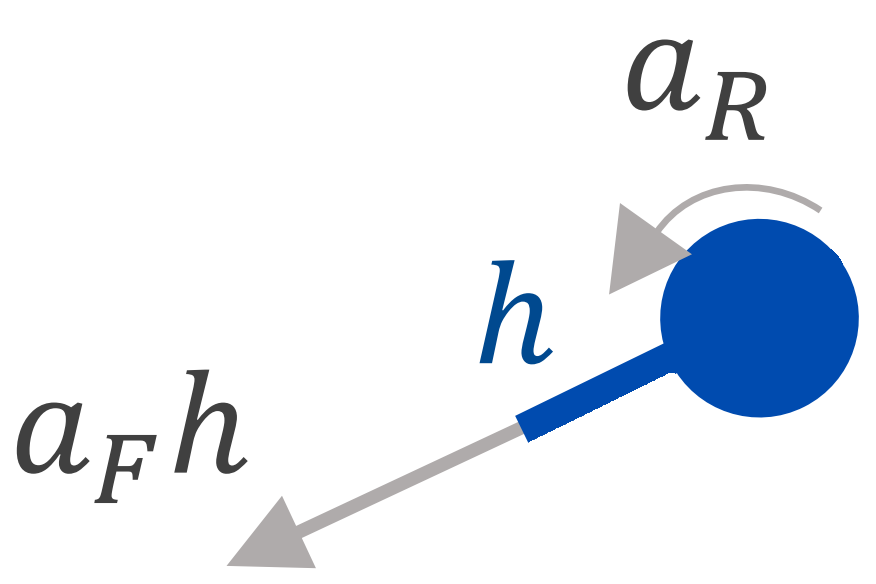
\includegraphics[width=\textwidth]{agent_active.png}
        %\caption{Active forces.}
        %\label{fig:image1}
    \end{minipage}
    \hspace{0.1cm}
    \begin{minipage}{0.25\textwidth}
        \centering
        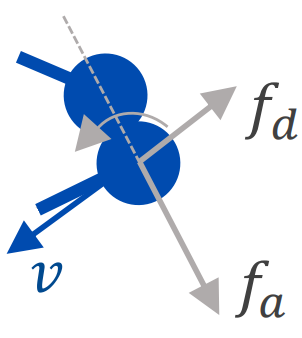
\includegraphics[width=\textwidth]{agent_passive.png}
        %\caption{Passive forces.}
        %\label{fig:image2}
    \end{minipage}
    \caption{Active (left) and passive (right) agent forces. \cite{li2023predator}}
    \label{fig:main_figure}
\end{figure}

To tailor the framework to our objectives, several modifications were implemented. These include:
\begin{enumerate}
    \item Agent visualization (unicycle to ant) and movement parameters (more "ant-like").
    \item Agent environment perception includes health status of the perceived agents.
    \item Keeping track of agent interactions, used for network evaluation.
    \item Redefine the reward policy to align with our disease-spread mitigation goals.
\end{enumerate}

\subsection{Basic Reward Policy}

Our initial reward policy aimed to produce social distancing patterns in agent behavior is based on direct collisions between agents as the primary form of information exchange. Collisions between agents of the same status (healthy-healthy or infected-infected) were rewarded to encourage grouping behavior. In contrast, collisions between agents of different statuses (healthy-infected or vice versa) were penalized to discourage close contact to limit disease spread.

The above mention policy is demonstrated in isolation with all healthy agents in Figure \ref{fig:demo}. On the left simulation we penalized each agent upon collision with a $-1$ reward, while on the right simulation we rewarded each colliding agent with a $+1$ reward. This demonstrates how a very simple change in the reward policy effects the learned behavior.

\begin{figure}[hbt]
    \centering
    \begin{minipage}{0.2\textwidth}
        \centering
        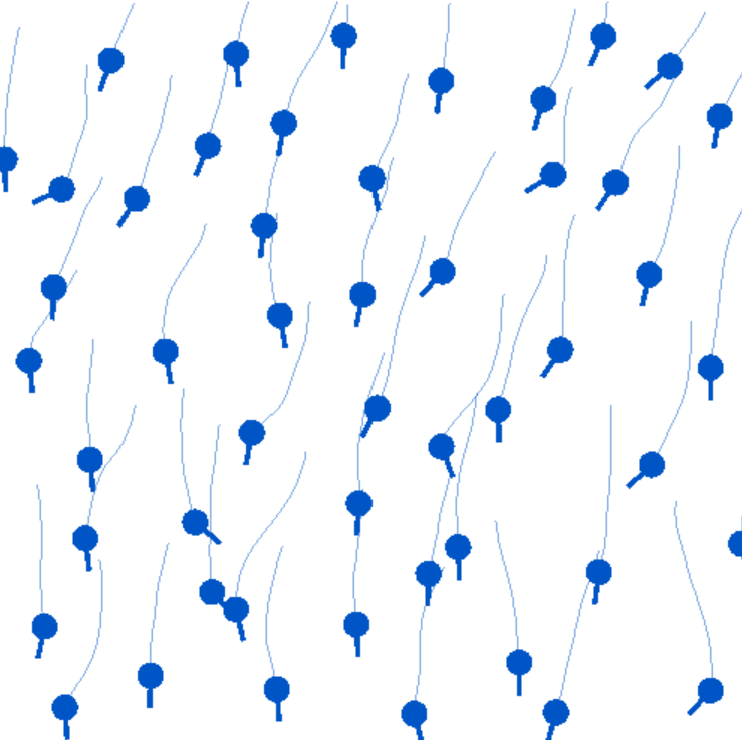
\includegraphics[width=\textwidth]{avoid.png}
    \end{minipage}
    \hspace{0.5cm}
    \begin{minipage}{0.2\textwidth}
        \centering
        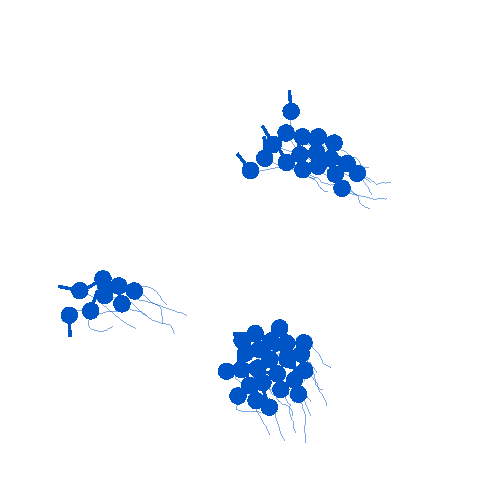
\includegraphics[width=\textwidth]{touch.png}
    \end{minipage}
    \caption{Demonstration of simple reward policies - penalize (left) or reward (right) collisions.}
    \label{fig:demo}
\end{figure}

We experimented with a diminishing reward system, where consecutive interactions were penalized progressively, which effectively prevented agent clustering: 
$$
\mathrm{reward}(a, b) = \begin{cases}
    -\lambda & \text{if } sick(a) \neq sick(b) \\ 
    +\sigma * \gamma (1 - recent(a,b)) & \text{otherwise.}
\end{cases}
$$
However, we ultimately decided not to include it in the final model, as it was considered overly engineered. 

To further enhance agent behavior, we introduced optional reward components that address specific aspects of agent-environment dynamics. These additions allow for greater adaptability to different scenarios:

\begin{enumerate}
    \item \textbf{Wall Collision Penalty} $\rightarrow$ In non-periodic environments, where agents encounter boundaries, a wall collision penalty discourages agents from colliding with walls:
    $$
    \mathrm{reward}(a) = \begin{cases}
        -\lambda & \text{if a collides with any wall}\\ 
        0 & \text{otherwise.}
    \end{cases}
    $$
    \item \textbf{Control Penalty} $\rightarrow$ To mimic energy consumption during movement, a control penalty was introduced. This reward is proportional to the magnitude of the agent’s control inputs ($aF$ for forward force and $aR$ for rotational force), encouraging agents to exhibit conservative movement:
    $$
    \text{reward}(aF, aR) = -(\alpha |aF| + \beta |aR|)
    $$
\end{enumerate}

These optional components offer additional flexibility to customize agent behavior for specific objectives while maintaining the simplicity and broad applicability of the core reward system. Together, the diminishing reward mechanism and optional components have proven effective in creating high-performing agents, with their interaction networks closely resembling real-world scenarios. Ant behavior serves as a key baseline for comparison, further validating the model's adaptability across various species and contexts.

Introducing an external task can enhance agent performance by adding complexity that more accurately reflects real-world dynamics, improving the model’s capacity to evaluate and simulate realistic agent interactions and responses to disease transmission. The external task we selected involves agents alternating between touching the left and right walls. Initially, each agent is randomly assigned a task to either touch the left or right wall. Agents are rewarded with +0.1 for moving in the correct direction and +1 for successfully reaching the assigned wall. Once an agent completes the task, it is switched to the opposite wall, prompting the agent to continuously adapt its movement strategy.

\subsection{Alternative Information Exchange}

Our main exploration of agent interaction (information exchange) was on the basis of collisions. As an alternative, we also considered a pheromone-based system inspired by ant behavior, where agents perceived "safety" or "danger" through accumulated, decaying concentrations. While promising in theory, this approach performed poorly compared to integrating movement-based tasks. The core issue was the lack of a clear relationship between pheromone observations and the actions needed to maximize rewards. This underscores the importance of designing observation mechanisms that directly guide actionable, reward-driven behavior.

\section{Results}

\subsection{Interaction Network Observations}

To assess whether social distancing behaviors emerge in agent interactions, we convert these interactions into a network and analyze its structure, following methods outlined in Stroeymeyt et al. (2018) \cite{Stroeymeyt2018}. During each evaluation step, interactions between agents are tracked and recorded in an $n \times n$ interaction matrix, where $n$ is the total number of agents. A collision between two agents is considered an interaction. After each evaluation, the interaction matrix is normalized to create the network. In this network, each node represents an agent, and edges are formed between nodes if their interaction value exceeds a threshold of 0.01. The interaction matrix values are used as edge weights, and each node is labeled with the agent's health status.

We tested our trained model by running an episode of 10,000 steps with both a random untrained network and a trained network. For each scenario, we constructed a network of all interactions during the episode to better understand the agent behaviors. In the random network, no clear structure emerged, and agents formed a nearly fully connected network. In contrast, the trained network showed emerging patterns, with infected agents interacting less with healthy ones but continuing to interact with other infected agents. 

This behavior aligns with our expectations. The separation in agent behavior becomes more apparent when edges are weighted based on the number of interactions between agents, providing a clearer representation of significant interactions. The resulting weighted network is displayed in Figure \ref{fig:filtered_net}.

\begin{figure}[hbt]
    \centering
    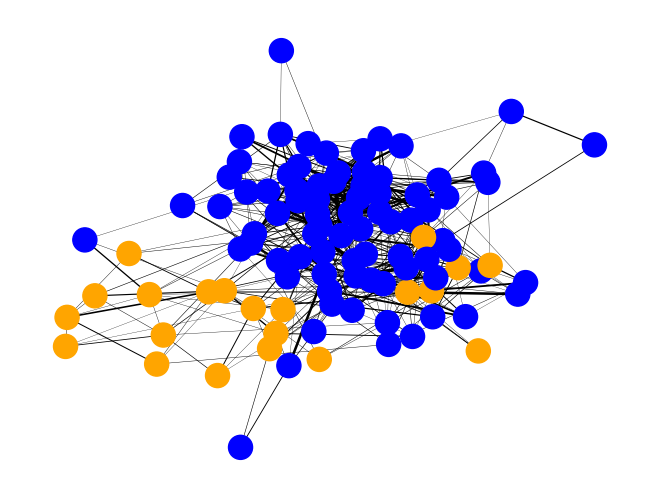
\includegraphics[width=0.9\linewidth]{filteredNet.png}
    \caption{Filtered learned interaction network.}
    \label{fig:filtered_net}
\end{figure}

This network is used to calculate relevant network measures such as clustering, modularity (between infected and non-infected agents), and network density, among others. These metrics help us better understand agent interactions. We anticipate that these metrics will increase as agents with the same health status interact more frequently within their respective groups.

In the filtered network, a clear trend emerges where infected agents interact significantly less with healthy agents. To gain deeper insights into these interactions and assess metrics beyond simple visual inspection, we analyzed key network properties related to pathogen transmission. Modularity increased from $-0.0005$ (in the random network) to $0.25$ (in the trained network), indicating greater separation between groups and denser clusters. This trend was further supported by a rise in clustering values from $0.056$ (random) to $0.066$ (trained). These changes suggest the emergence of basic social distancing behaviors, where infected and healthy agents reduce their interactions. Volz et al. (2011) \cite{volz2011effects} indicate that these properties contribute to reducing the spread of infection.

To explore pathogen-induced changes in network properties, we used our best-performing model and conducted $10$ experiments. In each experiment, we first designated certain agents as infected and performed a baseline evaluation episode of $10,000$ steps, during which no agents were actually infected. We recorded metrics such as clustering, modularity, and network efficiency. After this, we infected the designated agents and repeated the evaluation. The differences in these metrics before and after infection were then calculated to assess the impact of infection on network properties.

\begin{figure}[hbt]
    \centering
    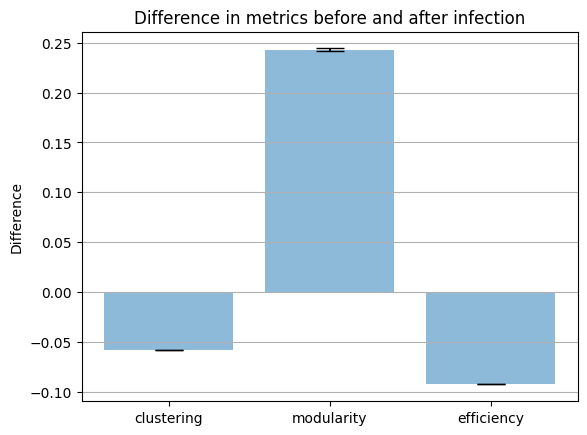
\includegraphics[width=0.9\linewidth]{figures/induced_changes.png}
    \caption{Changes in interaction network properties when introducing infected agents.}
    \label{fig:induced_changes}
\end{figure}

The results, shown in Figure \ref{fig:induced_changes}, reveal a significant increase in modularity, as infected agents became more segregated from the healthy population. Additionally, network efficiency decreased, suggesting an increase in the shortest paths within the network, which is consistent with reduced pathogen spread. However, contrary to expectations, clustering decreased. This anomaly can be explained by the initial lack of infected agents, resulting in a highly connected network with a high clustering coefficient of 0.138 due to the agents’ tendency to form dense groups.

\subsection{Simulation Visualization Observations}

\begin{figure}[hbt]
    \centering
    \begin{minipage}{0.2\textwidth}
        \centering
        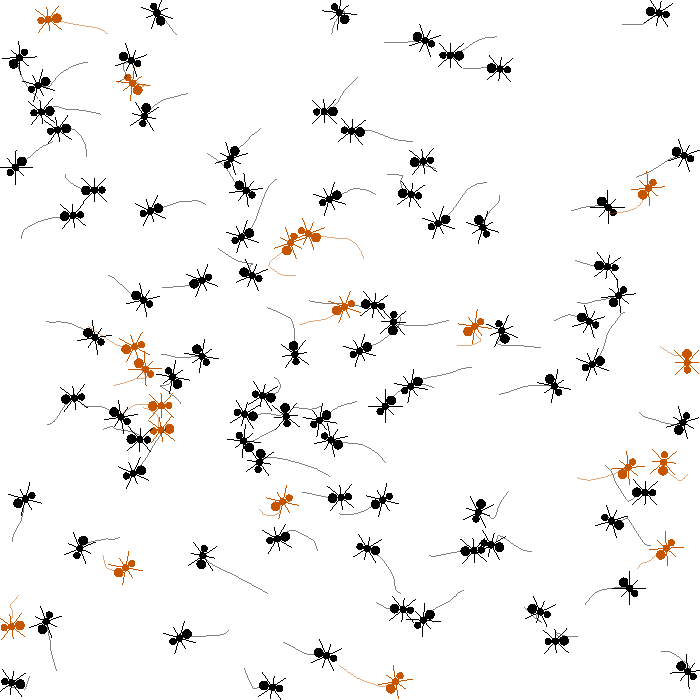
\includegraphics[width=.9\linewidth]{frame_25.png}
    \end{minipage}
    \hspace{0.2cm}
    \begin{minipage}{0.2\textwidth}
        \centering
        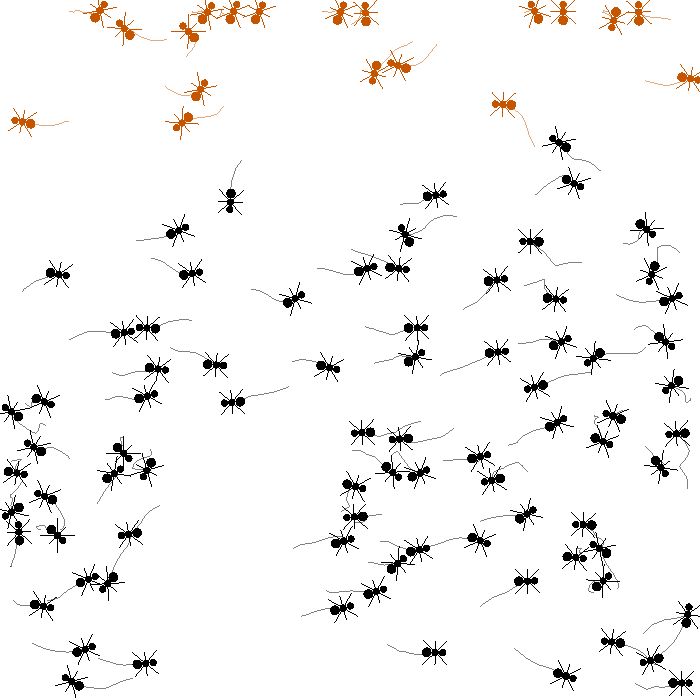
\includegraphics[width=.9\linewidth]{frame_1300.png}
    \end{minipage}
    \caption{Start of simulation (left) compared to end of simulation (right)}
    \label{fig:trained_viz}
\end{figure}

Figure \ref{fig:trained_viz} illustrates a simulation of our best-performing policy. Orange ants represent infected agents, while black ants represent healthy ones. The left image (frame 25) shows the start of the simulation, and the right image (frame 1300) depicts a later stage. A clear separation between the two groups is observed, minimizing contact between agents of different health statuses. Notably, this separation only emerged after introducing the additional left-to-right movement task. Without this task, while the interaction network properties remained similar, the visual separation was far less pronounced.

\section{Discussion}

In this study, we explored the use of reinforcement learning (RL) to model social distancing behaviors in artificial agents, focusing on minimizing disease transmission in a two-dimensional environment. Drawing inspiration from natural behaviors such as those observed in ants, agents exchanged health information and adapted their movements to avoid infected individuals, simulating social distancing. 

Results showed that agents trained with a basic reward policy for avoiding infected individuals successfully increased the separation between healthy and infected agents, as observed in interaction networks. Key network metrics, such as modularity and clustering, revealed clear segmentation between infected and non-infected agents, supporting the emergence of social distancing behavior. The network's increased modularity and clustering suggested that agents were minimizing disease transmission by avoiding contact with infected individuals. 

We also explored the effects of reward components, such as diminishing rewards, control penalties, and wall collision penalties, which further refined the agents’ behavior. These components enhanced adaptability, encouraging more efficient movement patterns and minimizing the risk of infection spread.

A key aspect of our model was the integration of an external task—agents alternating between touching left and right walls—which encouraged more structured behavior, facilitating social distancing. In contrast, a pheromone-based information exchange system was less effective due to its lack of direct alignment with reward-driven actions. This highlights the importance of designing reward systems that guide agent behavior towards the desired outcome. 

Our findings suggest RL can effectively model disease spread and social distancing behaviors. Future work can build on these findings by incorporating more complex disease transmission dynamics, improving agent interactions, and applying the model to real-world scenarios like public health simulations and swarm robotics.
\\

\noindent\textbf{CONTRIBUTIONS}: \textbf{LT} prepared/fixed the environment setup and did the basic avoid/touch experiments, \textbf{INS} and \textbf{AZ} did the reward policy experiments and the network statistics, \textbf{NL} did the alternative interactions experiment and organized/polished the report. Each member wrote their own parts of the report.

\printbibliography

\end{document}
